\ESKDappendix{обязательное}{Описание экспериментов по проверке состоятельности использованных методов локализации робота с помощью сторонней системы технического зрения}\label{app_cv_system}

Система технического зрения (СТЗ) представляет собой веб-камеру Logitech C920 FullHD закрепленную над зоной проведения экспериментов на высоте $2.85$ метра. Камера подключена к стационарному компьютеру, не связанному с роботом, на котором запускается программа на языке программирования Python. Для решения задач СТЗ используется библиотека OpenCV. На роботе закреплена плоская панель с двумя маркерами: синим -- над задней осью и красным -- в передней части робота. Центр масс синего маркера располагается над точкой $C$ (см. рисунок~\ref{img_kinematic_model_picture}).

СТЗ работает по следующему алгоритму:
\begin{enumerate}
	\item каждый из кадров видео-потока представляется в цветовом пространстве HSV (Hue, Saturation, Value);
	\item из кадра выделяются области с красным и синим цветам;
	\item вычисляются координаты маркеров в СК кадра;
	\item по расположению красного маркера относительно синего рассчитывается ориентация робота;
	\item значения координат и ориентация робота записываются в файл и выводятся на кадре.  
\end{enumerate}

Для проверка СТЗ был проведен эксперимент:
\begin{enumerate}
	\item при помощи отвеса и двух человек, камера была установлена так, чтобы оптическая ось была строго перпендикулярна плоскости пола зоны эксперимента;
	\item на полу были отмечены четыре точки и измерены расстояния между ними;
	\item последовательно в каждую точку ставился робот так, чтобы точка $C$ (или что то же самое -- центр масс синего маркера) была над отмеченной на полу точкой;
	\item фиксировался результат в виде скриншота с отмеченными на нем координатами робота. 
\end{enumerate}

Результаты работы СТЗ при проверке приведены на следующих изображениях.

\begin{figure}[h!]
	\begin{minipage}[h]{0.47\textwidth}
		\centering{ 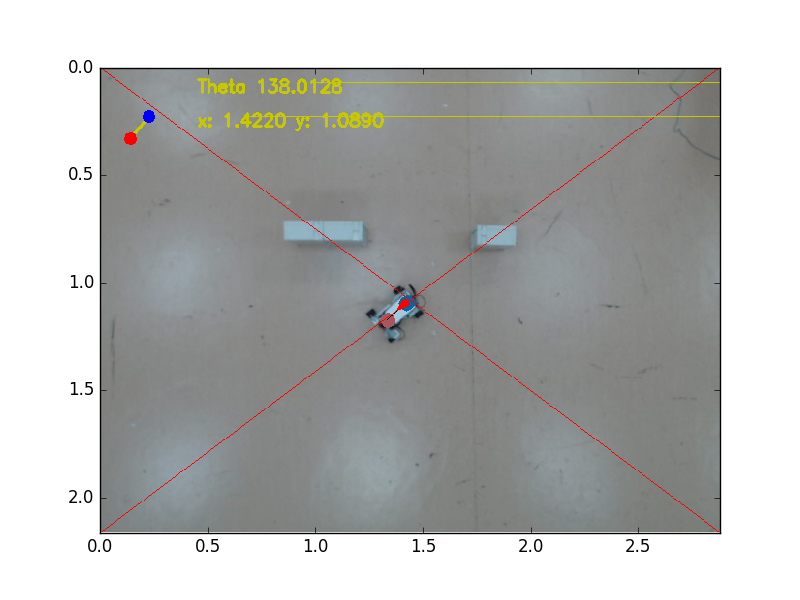
\includegraphics[width=\textwidth]{img/cv_2.png} \\ a) (1.422, 1.089)}
	\end{minipage}
	\hfill
	\begin{minipage}[h]{0.47\textwidth}
		\centering{ 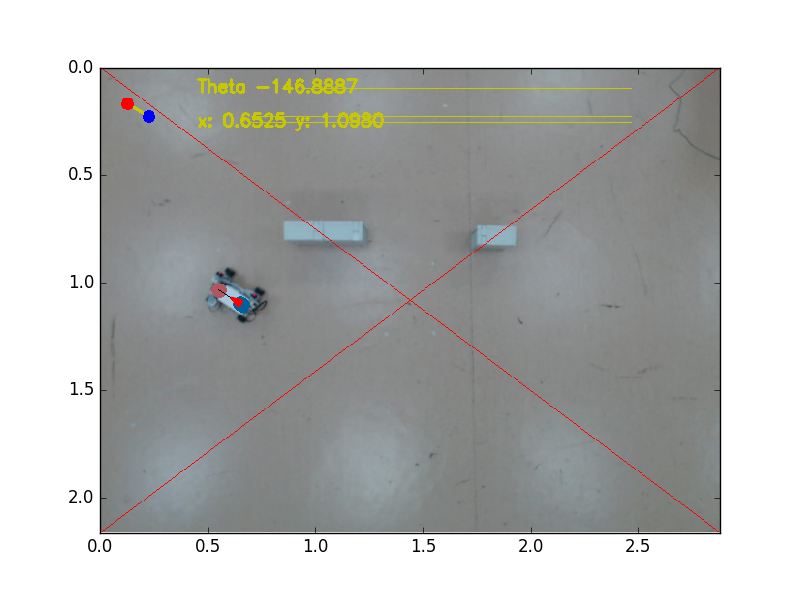
\includegraphics[width=\textwidth]{img/cv_3.png} \\ б) (0.6525, 1.098)}
	\end{minipage}
	\vfill
	\begin{minipage}[h]{0.47\textwidth}
		\centering{ 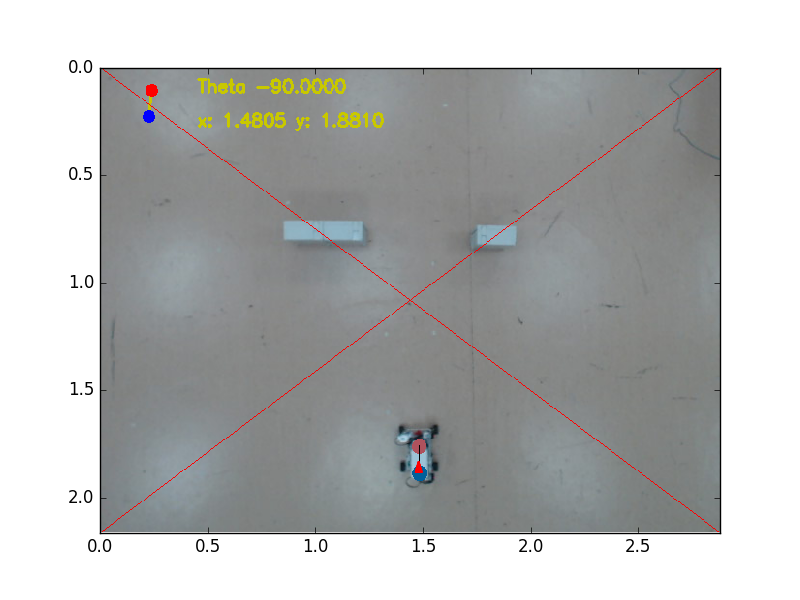
\includegraphics[width=\textwidth]{img/cv_1.png} \\ в) (1.4805, 1.881)}
	\end{minipage}
	\hfill
	\begin{minipage}[h]{0.47\textwidth}
		\centering{ 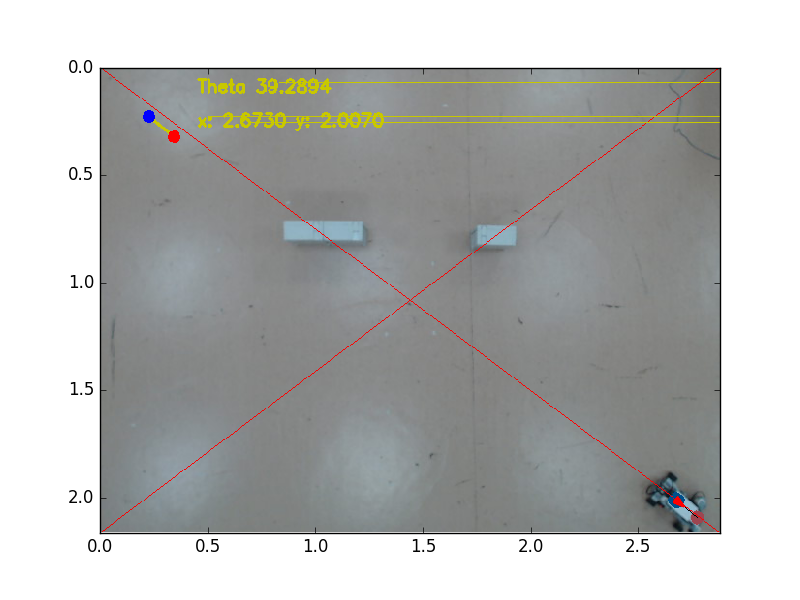
\includegraphics[width=\textwidth]{img/cv_4.png} \\ г) (2.673, 2.007)}
	\end{minipage}
	\caption{Проверка СТЗ.}
	\label{cv_check}
\end{figure}

Результаты проверки приведены в таблице~\ref{cv_check_results}.

\begin{table}[]
	\centering
	\caption{Результаты проверки СТЗ}
	\label{cv_check_results}
	\begin{tabular}{llll}
		\multicolumn{1}{c}{\begin{tabular}[c]{@{}c@{}}Расстояние \\ между точками\end{tabular}} & СТЗ, м & Линейка, м & Ошибка, м \\
		а и б & 0.7695 & 0,75 & 0.0194 \\
		а и в & 0.7941 & 0,75 & 0.0441 \\
		а и г & 1.5516 & 1,44 & 0.1116
	\end{tabular}
\end{table}

Траектория движения робота с СТЗ приведена на рисунке~\ref{cv_trajectory}
\begin{figure}[h]
	\centering
	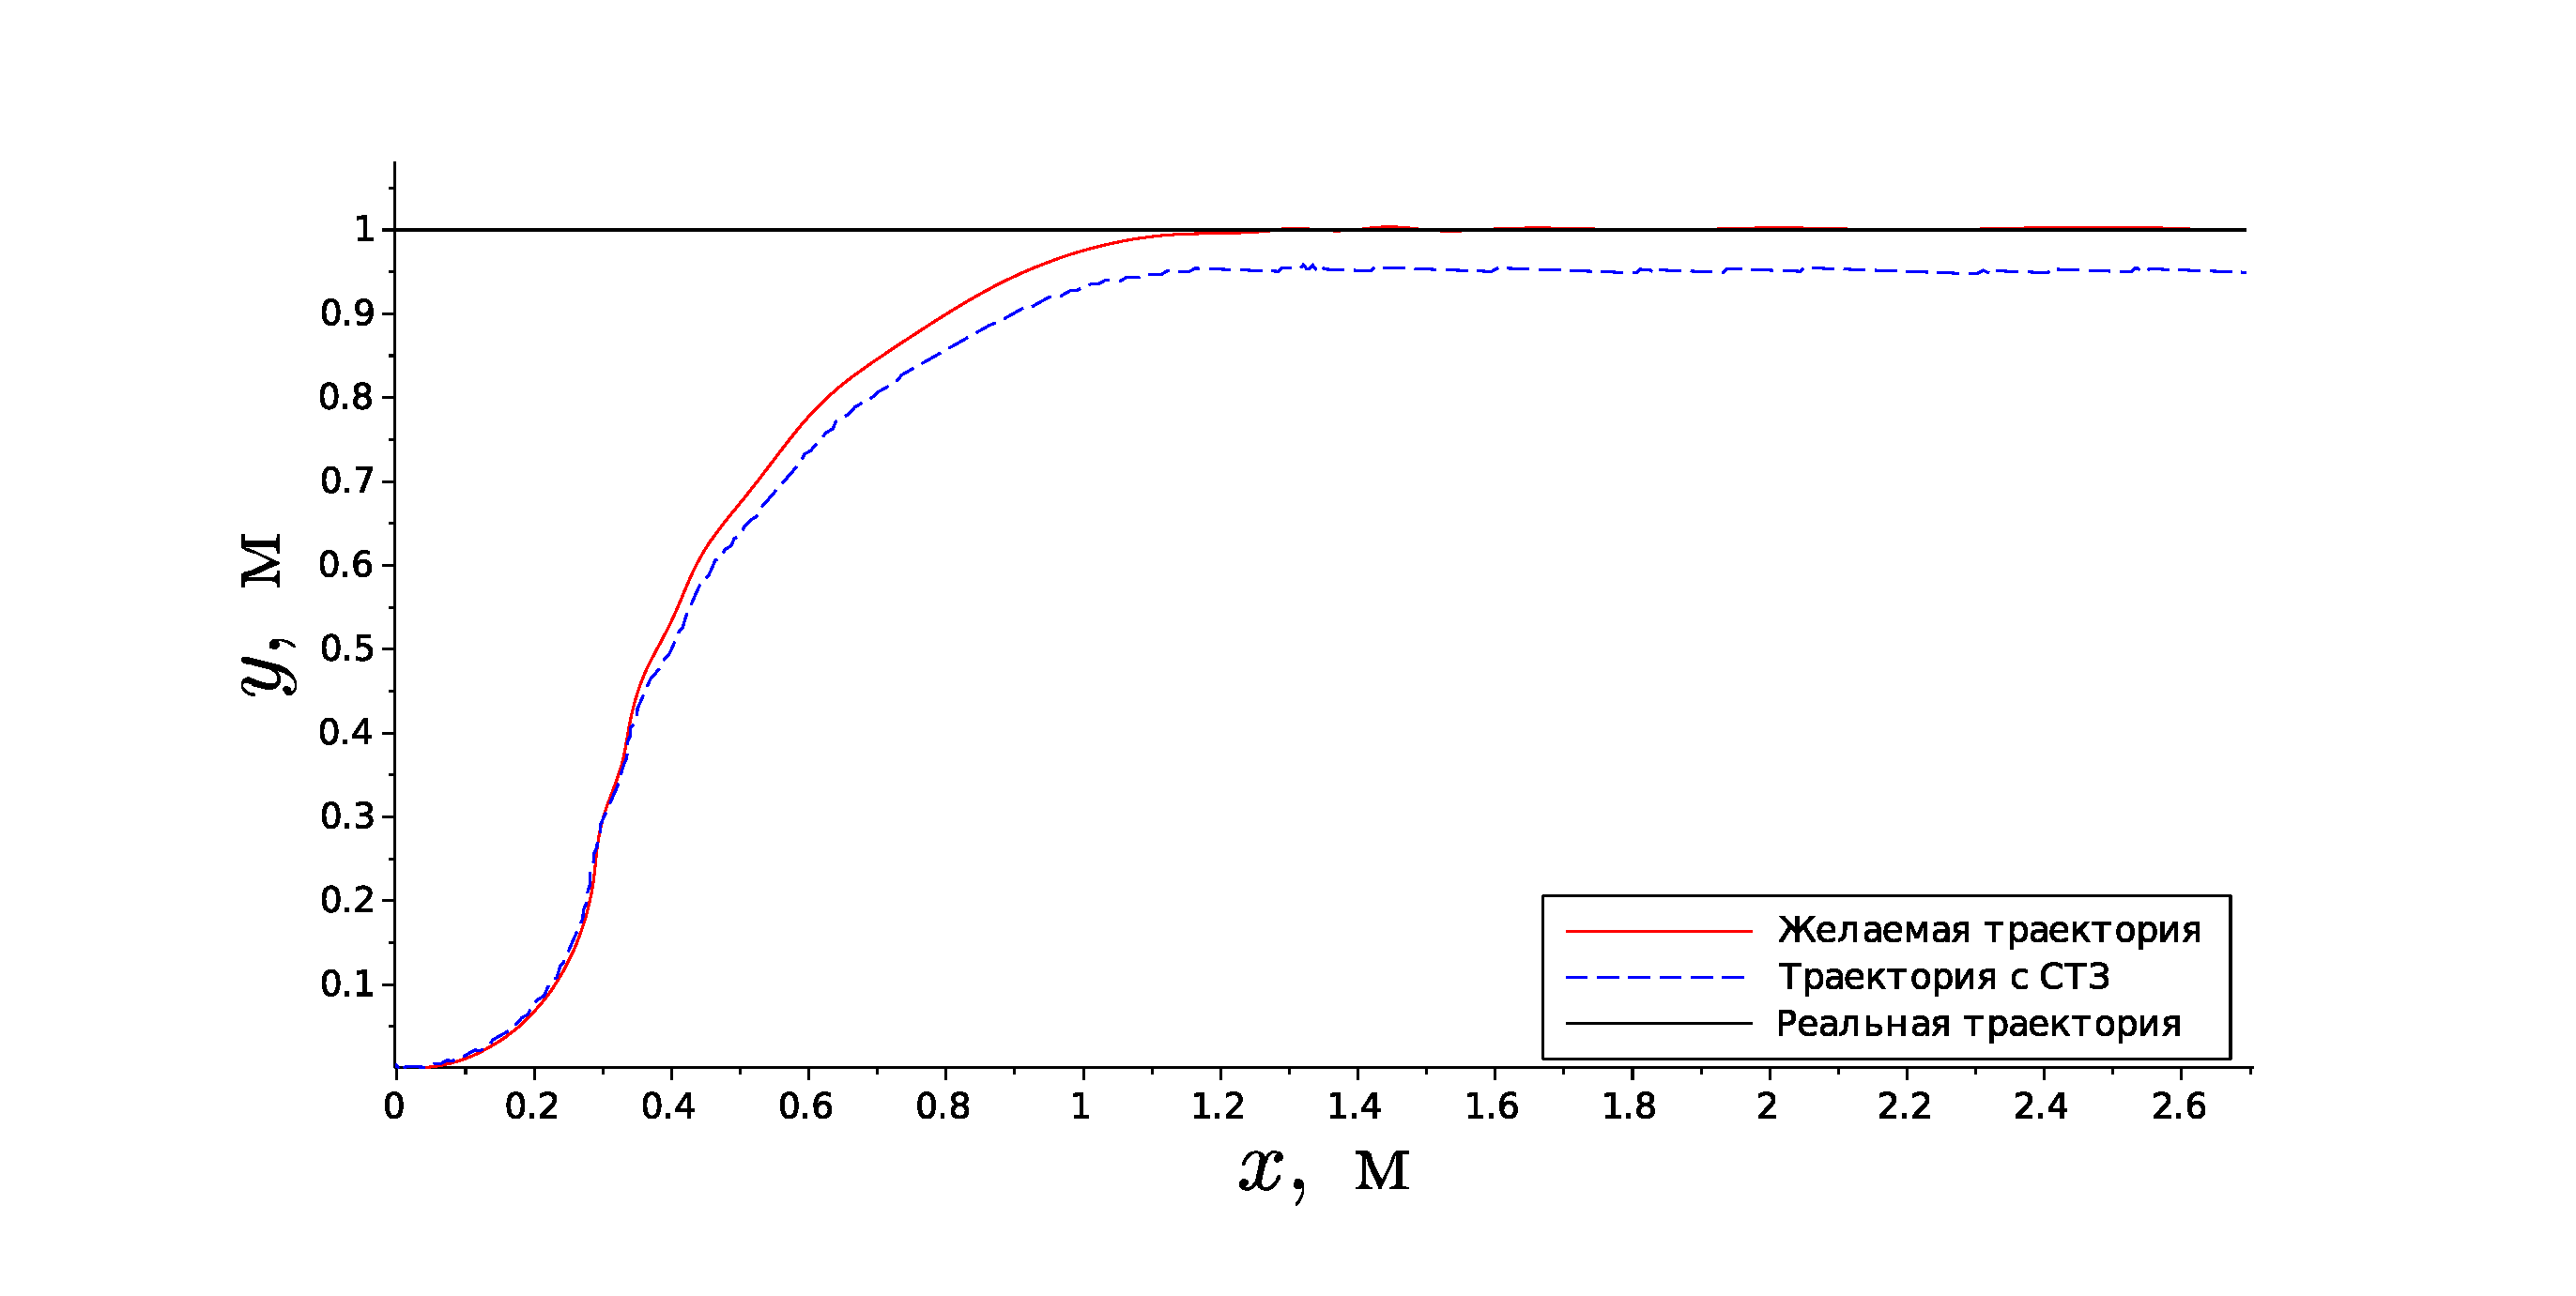
\includegraphics[width=\textwidth]{cv_trajectory.pdf}
	\caption{Траектория движения робота, полученная из СТЗ}
	\label{cv_trajectory}
\end{figure}

\begin{figure}[h]
	\centering
	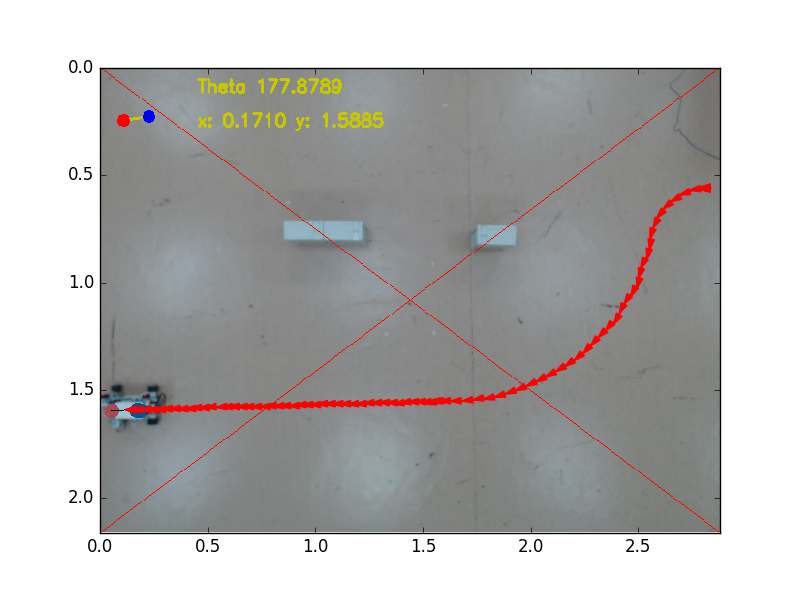
\includegraphics[width=0.9\textwidth]{cv_6.png}
	\caption{Траектория движения робота. Вид с камеры}
	\label{cv_trajectory_real}
\end{figure}